%
% Another appendix chapter
\chapter{Theoretic Limits on Capture}
It is hard, or even impossible, to find a closed-form solution of the state of a time-varying or nonlinear inverted pendulum model forward in time without introducing additional constraints, as discussed in Section \ref{sec:ewalking}. A common approach is to formulate an optimization problem, as for example in \cite{caron2018capturability}, to come to capture trajectory. However, few methods mention the limits achievable of the underlying model of the optimization problem. As convergence is often a problem in constrained nonlinear optimization, it could be useful to have a good guess of which states are achievable and which are not. In this chapter, limits on capture are given, considering constraints on height. As with the \ac{CP}, a point-foot, point-mass model is considered. Important constraints for this model are:
\begin{itemize}
	\item Unilateral \ac{GRF}.
	\item Limit on leg length or height.
	\item Limit on leg force.
	\item Limit on ground friction.
\end{itemize}
The latter two constraints are not considered in the following methods and therefore are the introduced points seen as limits or approximated effects, as they are likely not achievable with the true system.

 %% Capture Region
\section{Unconstrained Capture Region}
The search for the the new points is started off by finding a limit only under constraint of unilaterality of \ac{GRF}. Like with \ac{CP}, an initially horizontally traveling point-mass is considered. \\
The balistic touchdown time for a given height is for this point-mass:
\begin{equation}\label{eq:tbal}
	t_{balistic} = \sqrt{\frac{2z_0}{g}}.
\end{equation}
The horizontal touchdown location is:
\begin{equation}
	x_{balistic}= \dot{x}t=\dot{x}\sqrt{\frac{2z_0}{g}} 
\end{equation}
which is compares to the capture point as:
\begin{equation}
    x_{balistic}=\sqrt{2}x_{cp}
\end{equation}
This can also be reasoned from a leg force perspective, as no energy is substracted from the point-mass during its travel. Using this formulation and inserting a final velocity Equation \eqref{eq:Elip} gives:
\begin{equation}
   x_{balistic}^2 = \frac{z_0}{g}(\dot{x}_0^2 + \dot{x}_f^2), 
\end{equation}
where $\dot{x}_f$ is the final horizontal velocity of the \ac{CoM}. If a balistic trajectory is considered, the horizontal velocity is not affected until touchdown, so $\dot{x}_0=\dot{x}_f$. \\
To explain this with respect to a limit on the capture region: at thouchdown, the virtual leg can apply an impuls so that $\dot{x}_f$ becomes zero. After this, the point-mass can be risen to its original height again, without influencing the horizontal dynamics, which are zero. On the other side of the region, when to point-foot position is infinitely close to the point-mass, the virtual leg has to apply an infinite force to let the horizontal velocity become zero. After this, the point-mass can be lowered again to its default height. The region of between those two limits reads as follows:
\begin{equation}
\{x_{\dot{x}_f=0} \in (0, \dot{x}\sqrt{\frac{2z_0}{g}} ]\}.
\end{equation}
In \figref{fig:cpbal} this region and how this compares to the \ac{CP} is visualized. With grey plots, made with the method of \cite{koolen2016balance}, it can be observed how the trajectories can evolve approaching the limits. 

\begin{figure}[h]
\centering
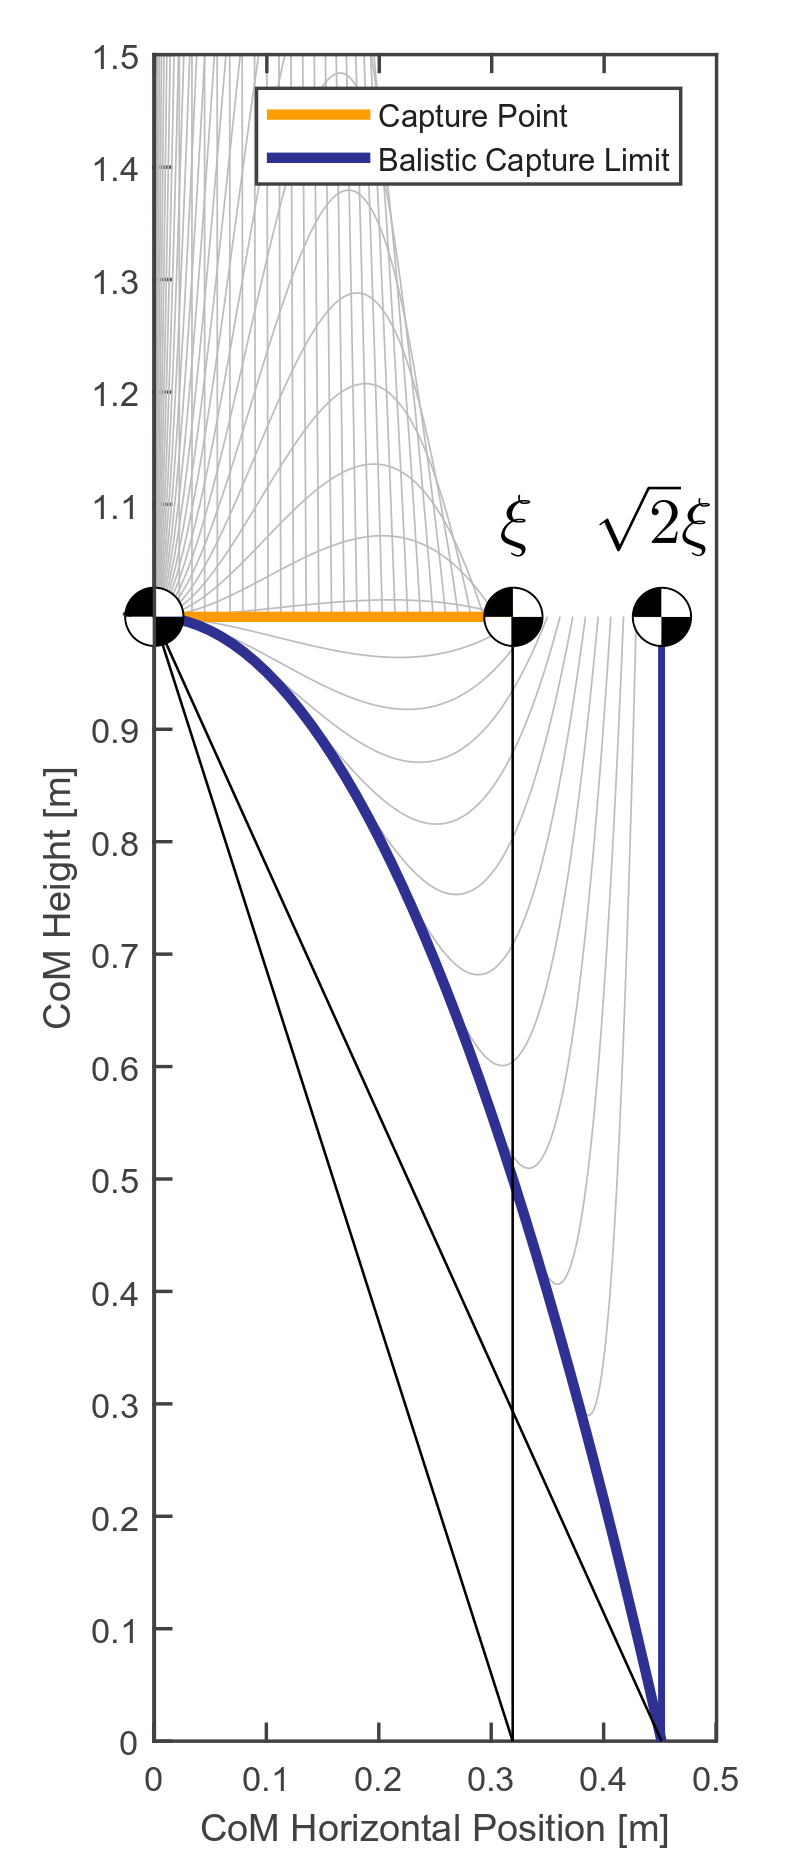
\includegraphics[width=0.3\textwidth]{STYLESTUFF/CPvsBalistic.png}
\caption{Unconstrained capture region and balistic limit. The grey plots visualize possible intermediate trajectories and are made with the method of \cite{koolen2016balance}}.
\label{fig:cpbal}
\end{figure}
\newpage
%% Impact influence
\section{Impact Influenced Capture}
To find the influence of the impact on capture, the question of the previous section is reversed: what does an nonzero negative height velocity do to the capturability, if it is directly stopped by an impact? To some extend, this has similarities to the work done in \cite{kuo2005energetic}. In the mentioned work, one of the goals is to find the energetic effects of the impacts of steps when a (nonlinear) inverted pendulum model is considered. In this section, the energetic influences are considered by direct trantioning to the \ac{CP} trajectory.\\
Consider a capture point where the initial horizontal velocity is increased by an impact:
\begin{equation}
x_{cp,impact} = \sqrt{\frac{z}{g}}(\dot{x}_0+\dot{x}_I),
\end{equation}
where $x_{cp,impact}$ is the impact influenced capture point and $\dot{x}_I$ is the added velocity generated by an impact. In the same way as in \eqref{eq:dotximpact}, this added velocity in terms of vertical velocity is written as:
\begin{equation}
x_{cp,impact} = \sqrt{\frac{z_0}{g}}(\dot{x}_0-\frac{x_{cp,impact}}{z_0}\dot{z}_I). 
\end{equation}
Under the assumption that the vertical velocity is driven to zero instantaneously by the impact, $\dot{z}_I=-\dot{z}_0$. Again, writing this point not as a function of itself, leads to:
\begin{align}\label{eq:xcpimpact}
x_{cp,impact} &= \frac{\sqrt{\frac{z_0}{g}}}{1+\frac{\dot{z}_I}{z_0}\sqrt{\frac{z_0}{g}}}\dot{x}_0,\\
			&= \frac{z_0}{\sqrt{z_0g}-\dot{z}_0}\dot{x}_0.
\end{align}

%% Height Constrained
\section{Height Constrained Capture}
If a time-varying model is considered for the capture point as in \cite{hopkins2014humanoid}, no closed form solution is possible. However, under the assumption that all height changes of the point-mass are generated by an initial impact generated by the virtual leg, the closed form solution is available. If this impact is either as early or as late as possible under the considered height constraint, it is a limit on capture for that particular height constraint. The more leg force is used farther from the virtual foot in horizontal direction, the more effect it has on the horizontal dynamics (Equation \eqref{eq:LIPeom}).\\
%minheight
\subsection{Minimum Height}
To calculate the limit under a minimum height constraint $z_{min}$, the point-mass has to fall until the constraint is reached, since the later the force is applied, the closer the point-mass is at its virtual base and the farther the mass can reach. Deriving from \ref{eq:tbal}, the balistic trajectory until the minimum height has as final height velocity:
\begin{equation}
	\dot{z}_{zmin} = -gt_{bal,z_{min}} = -g\sqrt{\frac{2\delta_{zmin}}{g}} = -\sqrt{2g\delta_{zmin}},
\end{equation}
where $t_{bal,zmin}, \dot{z}_{zmin}$ are the time and height velocity at the minimum height constraint and $\delta_{zmin}=z_0-z_{min}$. Plugging this height velocity in the impact influenced capture point of Equation \eqref{eq:xcpimpact} brings:
\begin{equation}
	x_{cp,impact}(z_{min}, \dot{z}_{zmin})= \frac{z_0-\delta_{zmin}}{\sqrt{(z_0-\delta_{zmin})g}+\sqrt{2g\delta_{zmin}}}\dot{x}_0.
\end{equation}
The capture point under a minimum height constraint is:
\begin{equation}
	x_{cp,minheight} =x_{bal,zmin}+x_{cp,impact}(z_{min}, \dot{z}_{zmin}) ,
\end{equation}
where  $x_{bal,zmin}$ is the horizontal position at the end of the balistic part. This results in the following equation for the capture limit under the minimum height constraint:
\begin{equation}
 x_{cp,minheight}=(\sqrt{\frac{2\delta_{zmin}}{g}} +\frac{z_0-\delta_{zmin}}{\sqrt{(z_0-\delta_{zmin})g}+\sqrt{2g\delta_{zmin}}})\dot{x}_0.
\end{equation}
In \figref{fig:cpzmin} the trajectory to this point is visualized.
%maxheight
\subsection{Maximum Height}
To calculate the initial impact as a function of the maximum height, there is looked at a simple kinetic and potential energy formula:
\begin{align}
 	\frac{1}{2}m\dot{z}_I^2 &= mg\delta z_{max},\\
 	\dot{z}_I &= \sqrt{2g\delta z_{max}},
\end{align}
where $\dot{z}_I$ is the generated vertical velocity by the impact and $\delta z_{max}$ is the height difference between the current and the maximum height, considering the initial vertical velocity is zero, as with the \ac{CP} \cite{pratt2006capture}. The initial horizontal velocity is influenced at the moment of impact as:
\begin{equation}\label{eq:dotximpact}
	\dot{x}_{0,I} = \dot{x}_0-\frac{x_{cp,height}}{z_0}\dot{z}_I,
\end{equation}
where $\dot{x}_{0,I}$ is the remaining horizontal velocity after impact and $x_{cp,height}$ is the capture point under the height constraint, to be determined. The way the height velocity $\dot{z}_I$ is calculated, assumes no external forces except for gravity $g$ in its calculation. As such, if the virtual leg would excert force during the time the vertical velocity after the impact $\dot{z}$ is nonzero, the height constraint $z_{max}$ would be violated. During the time $\dot{z}$ is driven to zero by gravity, the virtual leg force is considered to be zero. Under the motivation to find a limit on the closest possible point to come to a stop, the \ac{CP} is considered after the horizontal position where the $\dot{z}$ is driven to zero. In this way, the maximum leg force possible is used without violating the constraint $z_{max}$. Note that at the moment when $\dot{z}$ is zero, $\dot{x}_{0,I}$ is still the same value as just after the impact.\\
The time it takes until $\dot{z}$ is zero after the impact with zero leg force, is given by:
\begin{equation}
	t_{\dot{z}} =\frac{\dot{z}_I}{g},
\end{equation}
where $t_{\dot{z}}$ is the time that the height velocity is nonzero. With the proposed strategy, the capture point under maximum height constraint can be calculated the following way:
\begin{align}
	x_{cp,height}&=(t_{\dot{z}}+\sqrt{\frac{z_o+\delta z_{max}}{g}})\dot{x}_{0,I},\\
			&=(\frac{\dot{z}_I}{g}+\sqrt{\frac{z_o+\delta z_{max}}{g}})(\dot{x}_0-\frac{x_{cp,height}}{z_0}\dot{z}_I),
\end{align}
where $x_{cp,height}$ is the capture point under the constraint of $z_{max}$. Writing this expression not as a function of itself, leads to:
\begin{align}
	 (1+(\frac{\dot{z}_I}{g}+\sqrt{\frac{z_o+\delta z_{max}}{g}})\frac{\dot{z}_I}{z_0})x_{cp,height}& =		(\frac{\dot{z}_I}{g}+\sqrt{\frac{z_o+\delta z_{max}}{g}})\dot{x}_0,\\
	 x_{cp,height} & = \frac{(\frac{\dot{z}_I}{g}+\sqrt{\frac{z_o+\delta z_{max}}{g}})\dot{x}_0}{ 1+(\frac{\dot{z}_I}{g}+\sqrt{\frac{z_o+\delta z_{max}}{g}})\frac{\dot{z}_I}{z_0}}.
\end{align}
Finally, to write the point in terms of the initial state gives:
\begin{equation}
 x_{cp,height}  = \frac{\frac{\sqrt{2g\delta z_{max}}}{g}+\sqrt{\frac{z_o+\delta z_{max}}{g}}}{ 1+(\frac{\sqrt{2g\delta z_{max}}}{g}+\sqrt{\frac{z_o+\delta z_{max}}{g}})\frac{\sqrt{2g\delta z_{max}}}{z_0}}\dot{x}_0.
\end{equation}
In \figref{fig:cpzmax} the trajectory to this point is illustrated for  $\dot{x}_0=1.0$, $z_0=1.0$ and $z_{max}=1.1$, together with the capture point and a plot with the method of \cite{koolen2016balance}. Considering this 10\% height change, the capture limit is about $1-x_{cp}/x_{cp,height}\approx 10.37 \%$ closer than the \ac{CP} from the \ac{CoM}.
\begin{figure}[h]
\centering
  \begin{subfigure}{0.45\textwidth}
    \centering
  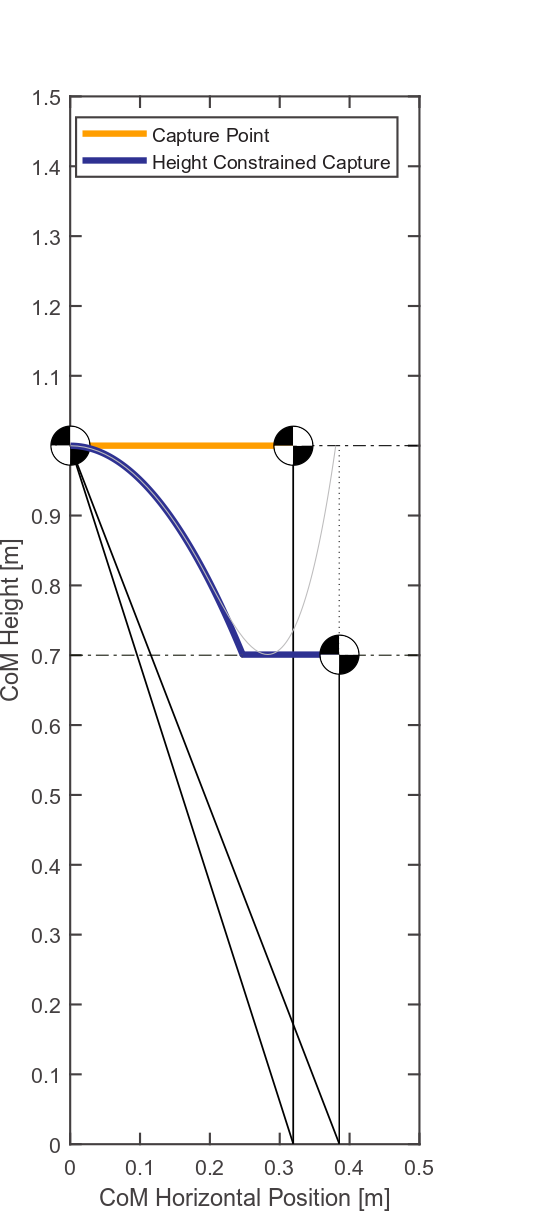
\includegraphics[width=.8\linewidth]{STYLESTUFF/CPvsMinHeight.png}
  \caption{}
   \label{fig:cpzmin}
  \end{subfigure}
  \begin{subfigure}{0.45\textwidth}
  \centering
  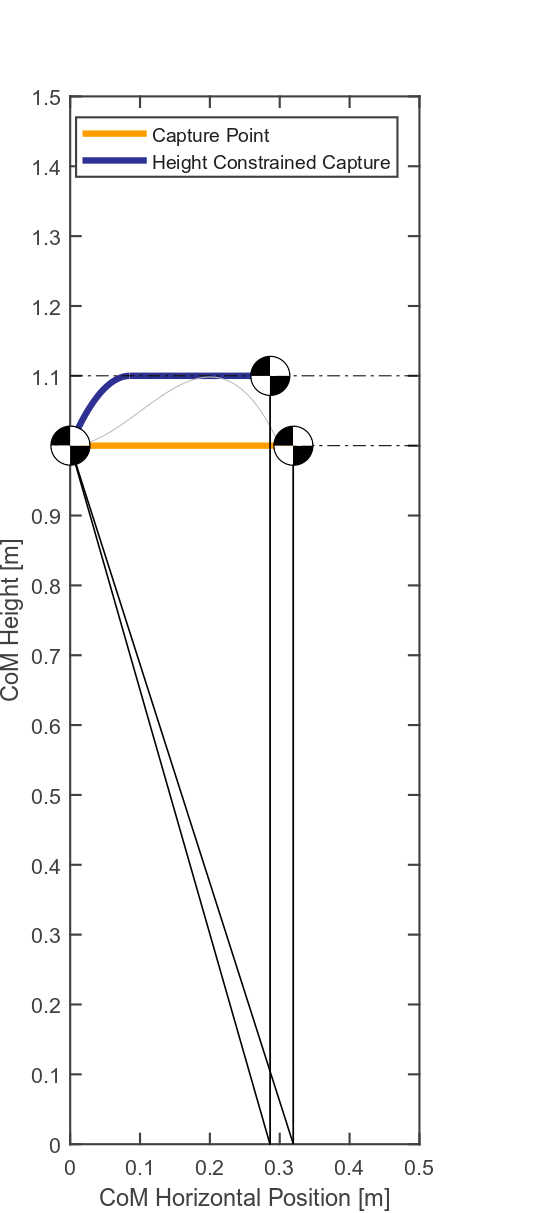
\includegraphics[width=.8\linewidth]{STYLESTUFF/CPvsHeight.png}
   \caption{}
    \label{fig:cpzmax}
  \end{subfigure}
  \caption{The height constrained capture limits for $\dot{x}_0=1.0$, $z_0=1.0$, (a) $z_{min}=0.7$ and (b) $z_{max}=1.1$. The grey plots are made with the method of \cite{koolen2016balance} and show that its final horizontal positions lie between the limit and the \ac{CP}. }
  \label{fig:cpz}
\end{figure}

%% Discussion
\section{Discussion}
In this chapter three different measures are proposed related to capturability of the point-mass, point-foot model, with an initial velocity that is horizontal. To summarize, these measures are:
\begin{itemize}
	\item A capture region or limit that only takes into account the unilaterality of contact constraint $\vect{f}_{leg}>0$.
	\item The closest possible capture location under a maximum height constraint $z_{max}$.
	\item The influence of an impact on the \ac{CP}.
\end{itemize}
These points or regions may not be of value for direct application, as they take a very limited amount of constraints into account on the model. However, just like with \ac{CP} and \ac{ICP}, they can be used for having an approximate guess of how the system dynamics will evolve over time. All of the proposed measures can be expressed in the systems current state and a maximum height constraint and are relatively computationally cheap compared to most optimization strategies, like trajectory optimization \cite{kelly2017introduction}.\\
The height constraint capture point might for example be used in an initial guess in an optimization algorithm, maybe factored down with a scaling value. The impact influence capture point can have value for motions where impacts at touch down can be expected beforehand, as for example in a planning or control strategy for robots that walk with straightened legs, as in \cite{griffin2018straight}. Moreover, as all three points are not dependent on any $y$-variable and can therefore be decoupled, they can be used without modification in \ac{3D} as well.